\documentclass{beamer}

% NOTE: reference
% https://arxiv.org/pdf/1604.05488.pdf

% HAGAR, first telescope to operate at an elevation > 4km
% http://www.tifr.res.in/~hagar/
% https://en.wikipedia.org/wiki/Indian_Astronomical_Observatory


\mode<presentation> {\usetheme{Madrid}}

\usepackage{graphicx}
\usepackage[utf8]{inputenc}
\usepackage{amsmath, amsthm, amssymb, mathtools}
\usepackage{hyperref}
\usepackage{flexisym}
\usepackage{mhchem}
\usepackage{textcomp}
\usepackage[export]{adjustbox}
\usepackage{subfig}
\graphicspath{{./img/}}

\title[TeV Astrophysics]{Astronomical facilities and instrumentation in TeV}

\author{Wei-Chih Huang}
\institute[NTHU]{
National Tsing Hua University \\
\medskip
}
\date{April 23, 2019}


\begin{document}

\begin{frame}{ICAT: MAGIC}
    Major Atmospheric Gamma Imaging Cherenkov Telescopes (MAGIC)
    \begin{figure}[h]
        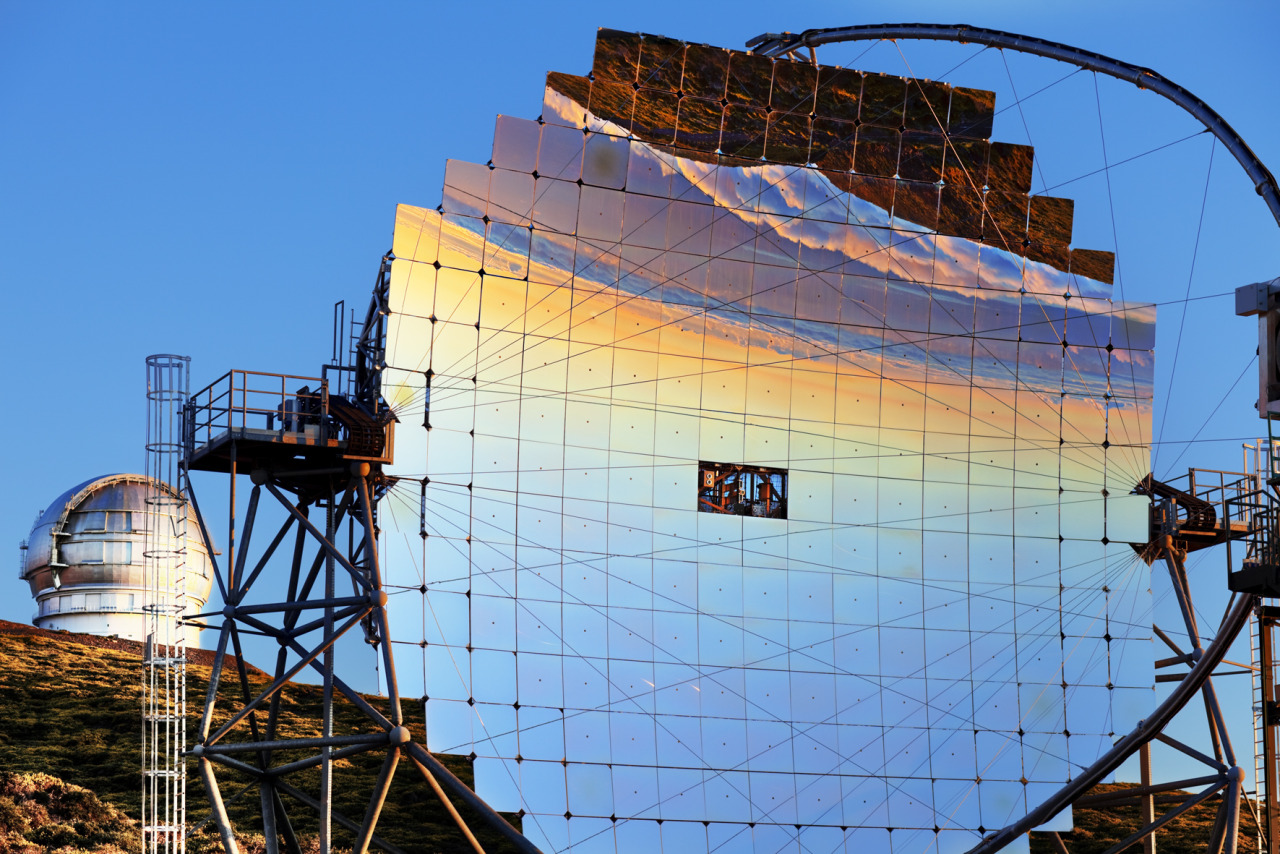
\includegraphics[width=280px]{MAGIC_mirror.jpg}
    \end{figure}
\end{frame}


\begin{frame}{ICAT: MAGIC}
    Location: 28 \textdegree45'43'' N, 17\textdegree53'24'' W at 2200 m
    \newline
    Detection method: Cherenkov technique
    \begin{figure}[h]
        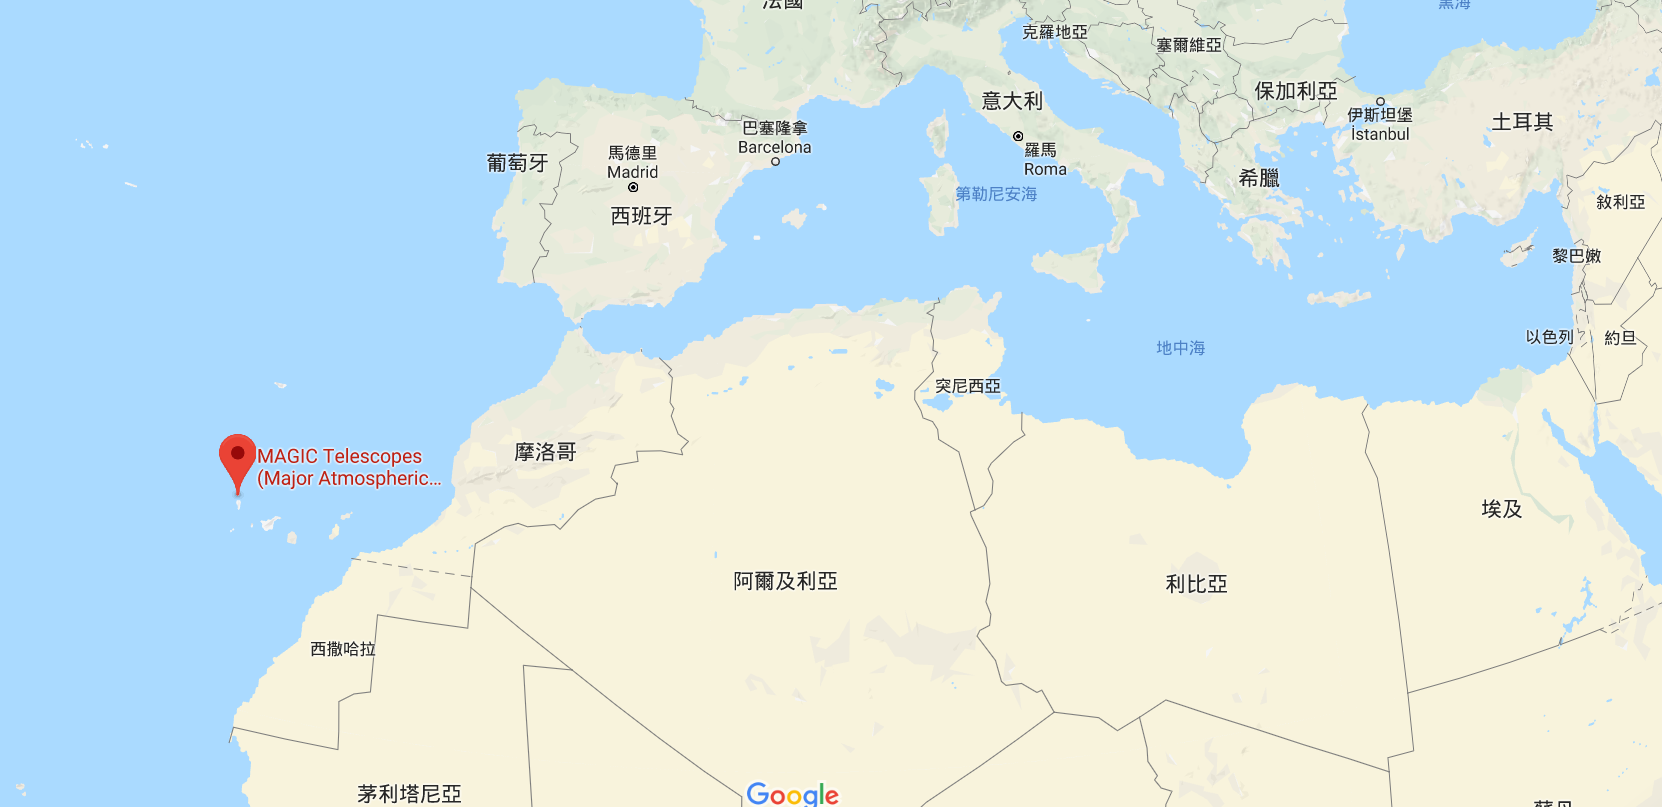
\includegraphics[width=280px]{MAGIC_location.png}
    \end{figure}
\end{frame}

\begin{frame}{ICAT: MAGIC}
    The first and most observed source is the Crab Nebula
    \begin{itemize}
        \item Accretion of black holes in active galactic nuclei
        \item Supernova remnants
        \item Other galactic sources such as pulsar wind nebulae or X-ray binaries
        \item Gamma ray bursts
        \item Unidentified EGRET or Fermi sources
        \item Annihilation of dark matter
    \end{itemize}
\end{frame}


\begin{frame}{ICAT: MAGIC}
    MAGIC I telescope component
    \begin{figure}[h]
        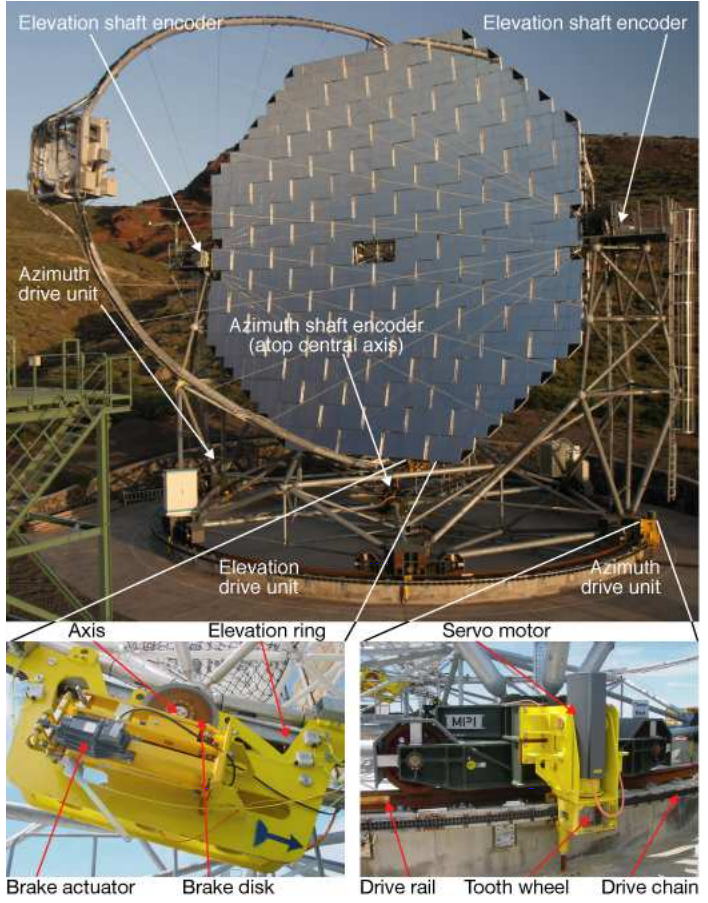
\includegraphics[width=165px]{MAGIC_I_component.png}
    \end{figure}
\end{frame}


\begin{frame}{ICAT: MAGIC}
	\begin{itemize}
		\item 150 scientists
		\item 20 scientific institutions
		\item over 20 different countries
    \end{itemize}
    \begin{figure}[h]
        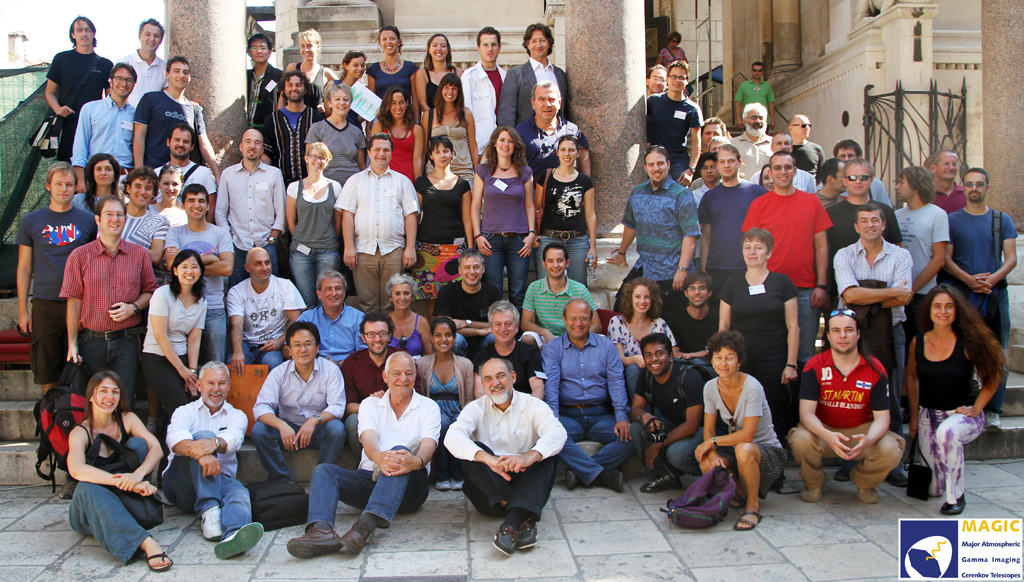
\includegraphics[width=280px]{CollaborationPicture2010.jpg}
        \caption{fall 2010 collaboration meeting in Split, Croatia}
    \end{figure}
\end{frame}


\begin{frame}{ICAT: MAGIC}
	Brief history:
	\begin{enumerate}
        \item mid-1994, project proposal
        \item 1998, construction started
        \item 2004, observation started
    \end{enumerate}
    \begin{figure}[h]
        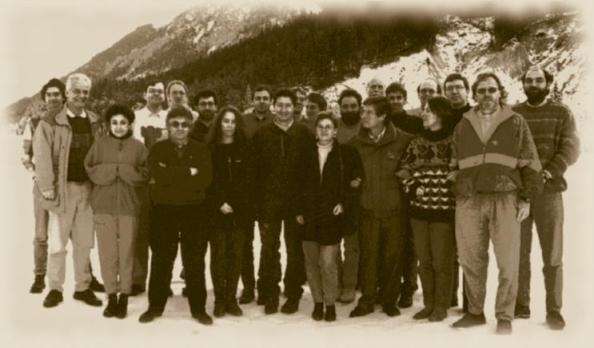
\includegraphics[width=230px]{magic-coll-old1.jpeg}
        \caption{A historic photo, from the beginning of our collaboration. It was taken at the first MAGIC design meeting, 1995, in The Eng, Austria.}
    \end{figure}
\end{frame}


\begin{frame}{ICAT: MAGIC}
    MAGIC-II vs MAGIC-I
    \begin{itemize}
        \item most fundamental parameters
        \item higher sensitivity
        \item Lower energy threshold
        \item higher QE photosensors
    \end{itemize}

    \begin{figure}[h]
        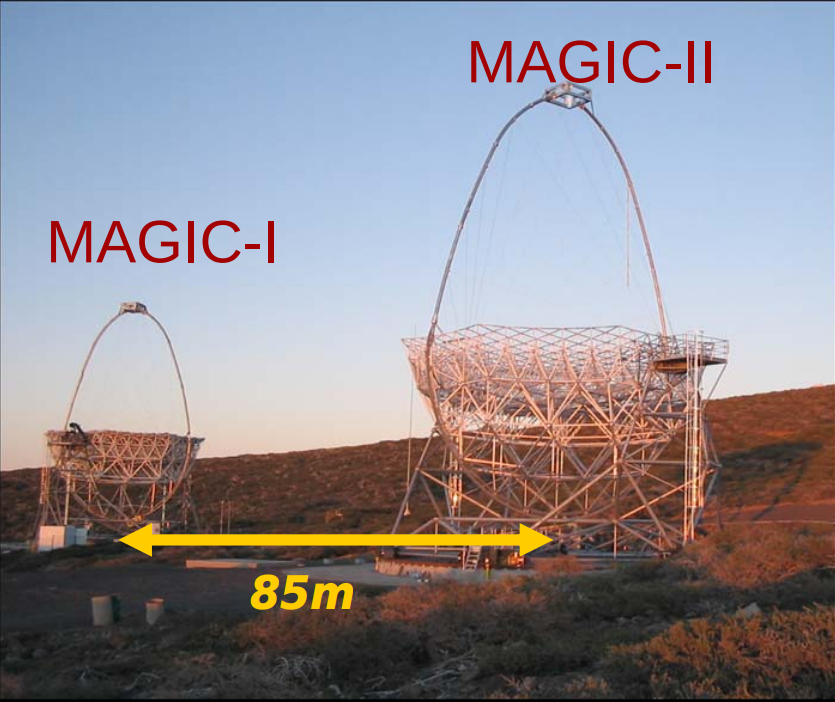
\includegraphics[width=250px]{MAGIC_12.png}
    \end{figure}
\end{frame}


\begin{frame}{ICAT: MAGIC telescope}
	\begin{itemize}
        \item Lightweight carbon fibre frame
        \item 396 separate hexagonal photomultiplier detectors in the center (diameter: 2.54 cm) surrounded by 180 larger photomultiplier detectors (diameter: 3.81 cm).
        \item Data are transferred in analogue form by fibre optic cables
        \item Signal digitization is done via an ADC (analog-digital converter) of frequency 2 GHz
        \item Total weight of 40,000 kg
        \item rotate 7 degrees per second
        \item energy range: 50GeV $\sim$ 50TeV
	\end{itemize}
\end{frame}


\begin{frame}{ICAT: MAGIC mirror}
    MAGIC-I:
	\begin{itemize}
        \item reflective mirror surface: 236 $\text{m}^2$ consisting of
        \item 956 50cm×50cm aluminium individual reflectors
        \item 13 kW heating system
    \end{itemize}
    \hfill \break
    MAGIC-II:
    \begin{itemize}
        \item 246 99cm×99cm mirror panels
        \item focal length to diameter ration is f/D = 1.03
    \end{itemize}

    \begin{figure}
        \centering
        \subfloat{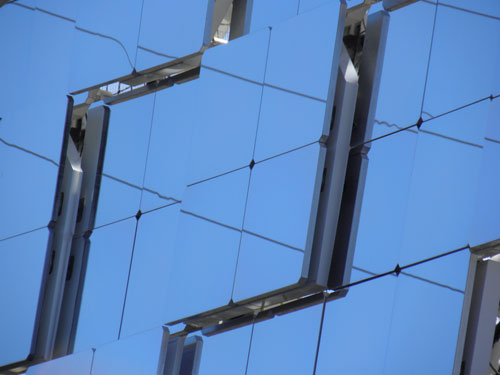
\includegraphics[width=130px]{MAGICMirror.jpg} }
        \qquad
        \subfloat{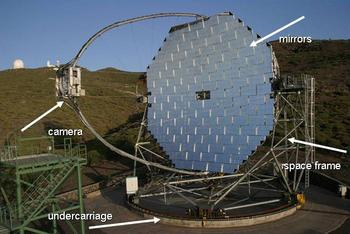
\includegraphics[width=120px]{MAGIC_telescope.jpg} }
    \end{figure}
\end{frame}


\begin{frame}{ICAT: MAGIC camera}
    \begin{itemize}
        \item 1039 photomultiplier tubes(both MAGIC telescopes)
        \item view: 3.5 degree
    \end{itemize}

    \begin{figure}
        \centering
        \subfloat{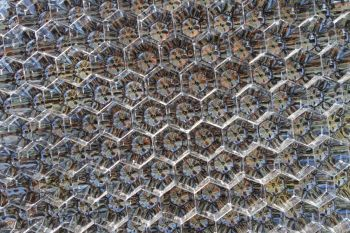
\includegraphics[width=130px]{MAGIC_PMTs.jpg}}
        \qquad
        \subfloat{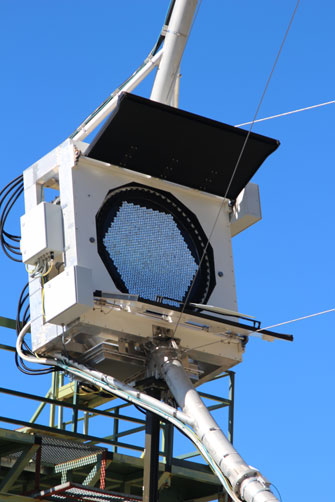
\includegraphics[width=120px]{MAGIC_Camera.jpg}}
    \end{figure}
\end{frame}


\begin{frame}{ICAT: MAGIC camera}
    \begin{figure}[h]
        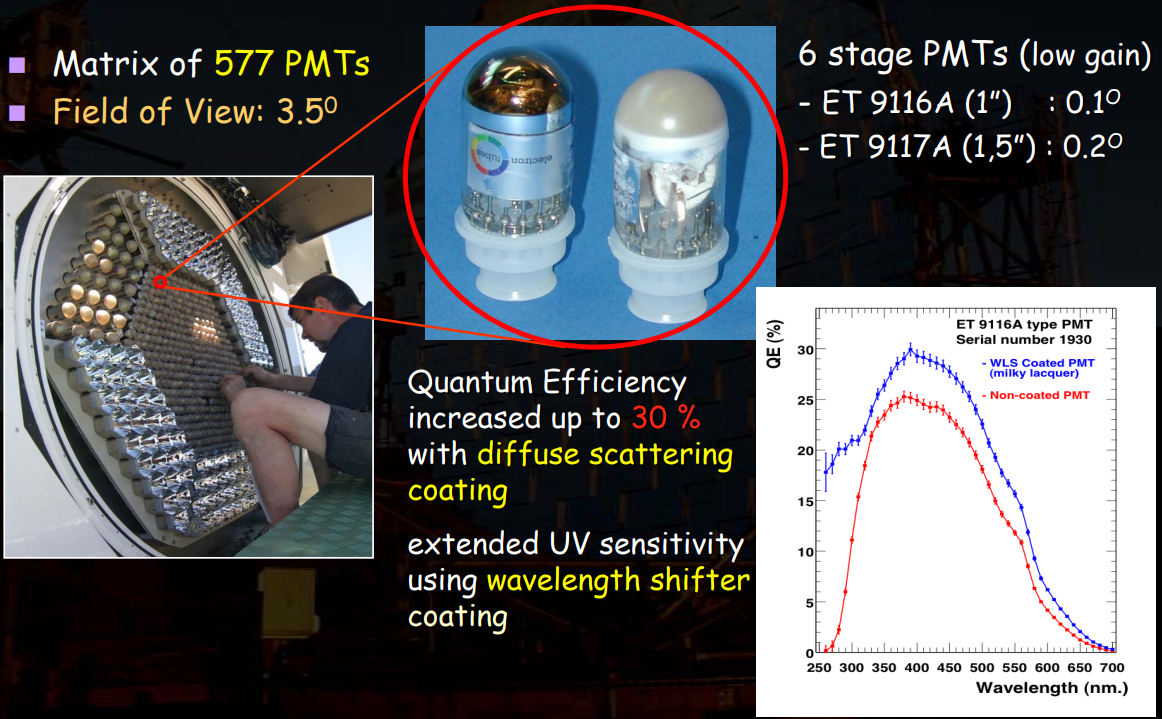
\includegraphics[width=300px]{MAGIC_PMTs.png}
    \end{figure}
\end{frame}


\begin{frame}{ICAT: MAGIC}
    MAGIC result:
    \begin{itemize}
        \item Discovered several galactic and extra-galactic sources
        \item Addresses many exciting physics topics
    \end{itemize}
\end{frame}

\end{document}